% \documentclass[a4paper, 10px]{ctexart}
\documentclass{ctexart}
\usepackage[left=1in, right=1in, top=1.2in, bottom=1.2in]{geometry}
\usepackage{ctex}
\usepackage[utf8]{inputenc}
\usepackage{boxproof}
\usepackage{fontspec}
\usepackage{a4wide}
% \setmainfont[Scale = 1]{SF Display}
% \setCJKmainfont{Songti SC}
\usepackage{fancyhdr}

% Automata
\usepackage{tikz}
\usetikzlibrary{automata, positioning, arrows}

\pagestyle{fancy}
\fancypagestyle{plain}{
    \fancyhead[L]{East China Normal University}
    \fancyhead[R]{}
    \fancyfoot[C]{\thepage}
}

\tikzset{
->, % makes the edges directed
>=stealth, % makes the arrow heads bold
node distance=3cm, % specifies the minimum distance between two nodes. Change if necessary.
every state/.style={thick, fill=gray!10}, % sets the properties for each ’state’ node
initial text=$start$, % sets the text that appears on the start arrow
}

\def\premise{\mathrm{premise}}
\def\assumption{\mathrm{assumption}}
\def\MT{\mathrm{MT\ }}
\def\LEM{\mathrm{LEM}}
\def\intro{\mathrm{i\ }}
\def\elim{\mathrm{e\ }}
\def\introa{\mathrm{i_1\ }}
\def\elima{\mathrm{e_1\ }}
\def\introb{\mathrm{i_2\ }}
\def\elimb{\mathrm{e_2\ }}

\title{Computation Theory Assignment 4}
\author{10185101210 陈俊潼}
\date{September 2020}

\begin{document}

\maketitle

\section{Automata}

\subsection{This is an automata.}

To draw an automata, you need to first import \texttt{tikz} package.

Figure \ref{aut1} is an example:


\begin{figure}[ht]
    \centering
    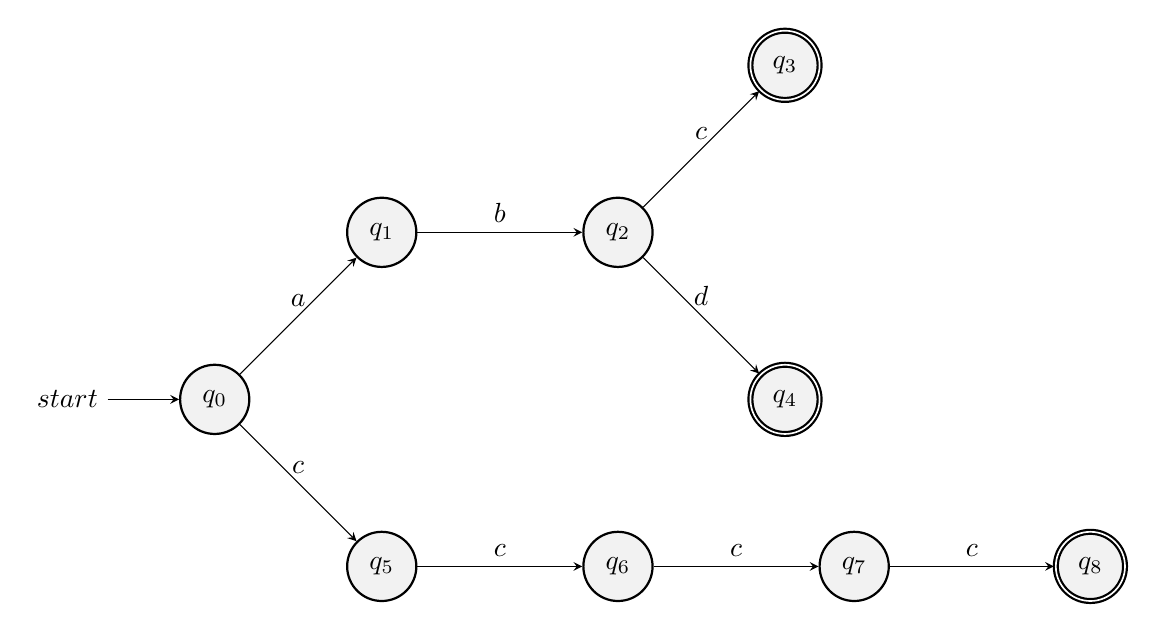
\begin{tikzpicture}[scale=2]
        \node[state, initial] (0) {$q_0$};
        \node[state, above right of=0] (1) {$q_1$};
        \node[state, right of=1] (2) {$q_2$};
        \node[state, above right of=2, accepting] (3) {$q_3$};
        \node[state, below right of=2, accepting] (4) {$q_4$};
        \node[state, below right of=0] (5) {$q_5$};
        \node[state, right of=5] (6) {$q_6$};
        \node[state, right of=6] (7) {$q_7$};
        \node[state, right of=7, accepting] (8) {$q_8$};
        \draw (0) edge[above] node{$a$} (1)
                (1) edge[above] node{$b$} (2)
                (2) edge[above] node{$c$} (3)
                (2) edge[above] node{$d$} (4)
                (0) edge[above] node{$c$} (5)
                (5) edge[above] node{$c$} (6)
                (6) edge[above] node{$c$} (7)
                (7) edge[above] node{$c$} (8);
    \end{tikzpicture}
    \caption{An automata example}
    \label{aut1}
\end{figure}
\end{document}
